\subsection{Analyseergebnis der obersten Ordnerebene}
\subsubsection{Übersicht der obersten Ordnerebene}
Die Quelltextdateien, welche die Anwendungen beschreibt, sind innerhalb des Ordners \lstinline|src| organisiert. 
% Die obersten Ordnerebene des \emph{src}-Ordner spiegelt die Architektur der Anwendung auf höchster Ebene wider.
Abbildung \ref{fig:obersteOrdnerebene} stellt die Zusammenhänge der obersten Ordnereben innerhalb des Ordners als Abhängigkeitsgraph dar. 
% Wird innerhalb eines Ordners Quelltext aus einem benachbarten Ordner importiert, wird dies durch eine Pfeilspitze am benachbarten Ordner gekennzeichnet. Beispielsweise importiert Quelltext innherhalb des Ordners \lstinline|designToSvgCLI| Quelltext aus dem Ordner \lstinline|core|.
\begin{figure}[H]
	\centering
    \caption{Übersicht der obersten Ordnerebene innherhalb des Ordner \lstinline|src|}
	\label{fig:obersteOrdnerebene}
	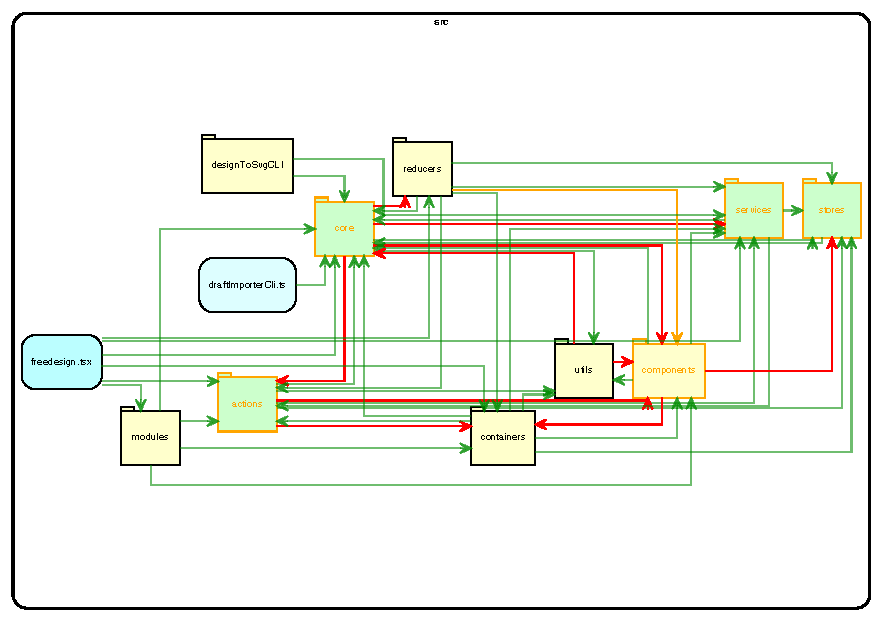
\includegraphics{diagrams/Ist-Architektur/Projektuebersicht.pdf}
\end{figure}

Der Abhängigkeitsgraph zeigt sämtlichen Ordner die im Ordner \lstinline|src| enthalten sind, so wie die TypeScript-Dateien \lstinline|freedesign.tsx| und \lstinline|draftImporterCli.tsx|, die ebenfalls im Ordner \lstinline|src| hinterlegt sind.  

Durch die Pfeile werden die Abhängigkeiten der Komponenten gekennzeichnet. Die Pfeilspitze zeigt auf den Ordner, auf des Inhalt Zugriffe erfolgen. Beispielsweise greift Quelletext im Ordner \lstinline|designToSvgCLI| auf Quelletext aus dem Ordner \lstinline|core| zu.
Wird eine Abhängigkeit durch das \lstinline|allowed|-Array bestätigt, wird diese durch einen grünen Pfeil dargestellt. Eine Abhängigkeit die durch das \lstinline|forbidden|-Array erfasst wird, wird durch einen roten Pfeil gekennzeichnet. Wird eine Abhängigkeit durch keine der beiden Arrays erfasst, wird diese durch einen orangen Pfeil dargestellt.

Enthält ein Ordner ungenutzten Quelltext, wird dies durch einen orangen Rahmen und einer orangen Bezeichnung gekennzeichnet.

\subsubsection{Ordnerinhalt der obersten Ordnerebene}
\paragraph{Der Ordner core} ist für den Anwendungskern vorgesehen und enthält Geschäftslogik sowie grundlegende Funktionalitäten und Datenstrukturen der Anwendung. 
Es ist vorgesehen, dass umgebender Quelletext auf den Quelltext des \lstinline|core|-Ordners zugreifen darf, jedoch ist der Zugriffe aus dem \lstinline|core|-Ordner heraus auf den umgebenden Quelletext untersagt. Dem Ordner mangelt es an einer klaren Strukturierung, auf Grund dessen die das richtig Zuordnung und Auffinden der Geschäftslogik schwierig ist. 

\paragraph{Im Ordner components} sind sämtlichen React-Komponenten zur Erzeugung der grafischen Oberfläche enthalten. Darunter zählen Komponenten zur Erzeugung von Menüs, Dialogen oder auch Werkzeuge zu Designbearbeitung. Die Komponenten besitzen keine Verbund zum \emph{Redux-State} und rufen keine \emph{Redux-Actions} auf. Die Komponenten können bei der Verwendung mit Eigenschaften versehen werden und damit an Redux gebunden werden. Dadurch ist das Verwenden der React-Komponenten in unterschiedlichen Kontexten möglich.

\paragraph{Der Ordner containers} enthält Komponenten (Container-Komponenten), welche die \emph{ReactJS}-Komponenten aus dem Ordner \lstinline|{components| mit den \emph{Redux-State} sowie \emph{Redux-Actions} verbindet. Somit verbinden die Container-Komponenten die grafische Oberfläche der Anwendung mit Redux.

% Ein Beispiel hierfür ist der \emph{Container} \lstinline|LoginDialog.tsx|, welcher das Anmeldeformular für die Kundenanmeldung erzeugt. Dieser nutzt Formularelemente und Schaltflächen aus dem \emph{components}-Ordner zur Erzeugung der grafischen Oberfläche. Für die Prüfung, ob der Kunden erfolgreich angemeldet ist, greift der Dialog auf die Kundendaten zu, die im \emph{Redux-State} verwaltet werden. Über eine \emph{Redux-Action} wird die Anmeldung durchgeführt, welche vom \emph{Container} aufgerufen wird. Dadurch das die grafischen Formularelement und Schaltflächen nicht an den Anwendungszustand gebunden sind, konnten sie z.B. auch in einem Dialog zur Kundenregistrierung verwendet werden.


\paragraph{Die Ordner reducers, action und stores} beziehen sich auf Redux und enthalten die Redux-Reducer, die Redux-Actions sowie den Redux-State. Der Redux-States ist auf mehrere Dateien innerhalb des Ordners \lstinline|stores| aufgeteilt. Die Dateien beziehen sich auf unterschiedlich Teile der Anwendung. Beispielsweise wird der Zustand der grafischen Oberfläche in der Datei \lstinline|guiState.ts| verwaltet und der Zustand des Projektes, welches gestaltet wird, in der Datei \lstinline|productState.ts|. 


% Für die Kommunikation mit der API von Unitedprint wird das Modul \emph{redux-axios-middleware} eingesetzt. 
% Das Module ist eine \emph{Redux}-Middleware für die asynchrone HTTP-Kommunikation. HTTP-Anfragen werden durch den Aufruf von \emph{Redux-Actions} ausgelöst, ebenso werden \emph{Redux-Actions} nach eintreffender Antwort ausgelöst \autocite[vgl.][]{ReduxAxios}. Im Ordner \emph{services} sind die \emph{Redux-Actions} für die API-Aufrufe definiert. Desweiteren enthält der Ordner noch eine Serviceklasse zur Kommunikation mit Zwischenablage des Betriebssystems. Die Klasse ermöglicht das einfügen von Text aus der Zwischenablage in das Design, sowie das Kopier von Text aus dem Design in die Zwischenablage.

\paragraph{Im Ordner utils} befinden sich nur zwei TypeScript-Dateien. Wie bereits im Architektur-Workshop festgestellt, ist die Existenz dieses Ordners fragwürdig und wird durch die 
Soll-Architektur aufgelöst werden.  

\paragraph{Der Ordner modules} wird ebenfalls durch die Soll-Architektur aufgelöst, da er React- und Redux-Komponenten enthält, welche in die Ordner \lstinline|components| und \lstinline|containers| integriert werden können.

\paragraph{Im Ordner styles} sind globale \emph{CSS}-Definition untergebracht, die das optische Erscheinungsbild der Anwendung beschreiben. Die Definitionen werden ausschließlich Komponenten im Ordner \emph{components} verwendete. 


\paragraph{}Die Datei \emph{freedesign.tsx} ist die Startdatei des FreeDesign-Editors, über die das Programm betreten wird. Für das Kommandozeilen-Programm \emph{Draft-Importer}, zum Import der Designvorlagen, ist die Datei \emph{draftImporterCli.ts} als Startdatei vorgesehen. Im Ordner \emph{designToSvgCLI}-Ordner wurde ein weiteres Kommandozeilen-Programm implementiert, welches ebenfalls für den Import der Designvorlagen benötigt wird.


% \paragraph{Zugriffe}
% Die grünen Zugriffspfeile stellen erwartete Zugriffe dar und sind somit gewollte Kopplungen der Einzellkomponenten. Im Gegensatz dazu sind die roten und orangen Zugriffspfeile ungewollte Zugriffe und wurden mit der Zeit integriert. Bei den roten Zugriffen besteht außerdem das Problem, dass diese Zyklen erzeugen und damit gegen die Forderung an eine Architektur, zyklusfrei zu sein, verstoßen. 

% Es bestehe sowohl einzelne Zyklen, wie zwischen den Ordner \emph{core} und \emph{services} sowie Zyklengruppen. Ein Beispiel hierfür ist die Gruppe bestehend aus \emph{actions}, \emph{utils} und \emph{core}.
% Auch innerhalb der Ordner bestehe Zyklen wischen Unterkomponenten. 
% Insgerammt wurden 14 Zyklen festgestellt.

% \paragraph{Verwaister Quelltext}
% Innerhalb der orange gekennzeichneten Ordner befinden sich verwaiste Quelltextabschnitte, welche nicht aufgerufen werden. Solche Quelltextstellen können die Verständlichkeit des Quelltext einschänken. 


% \begin{figure}[H]
% 	\centering
% 	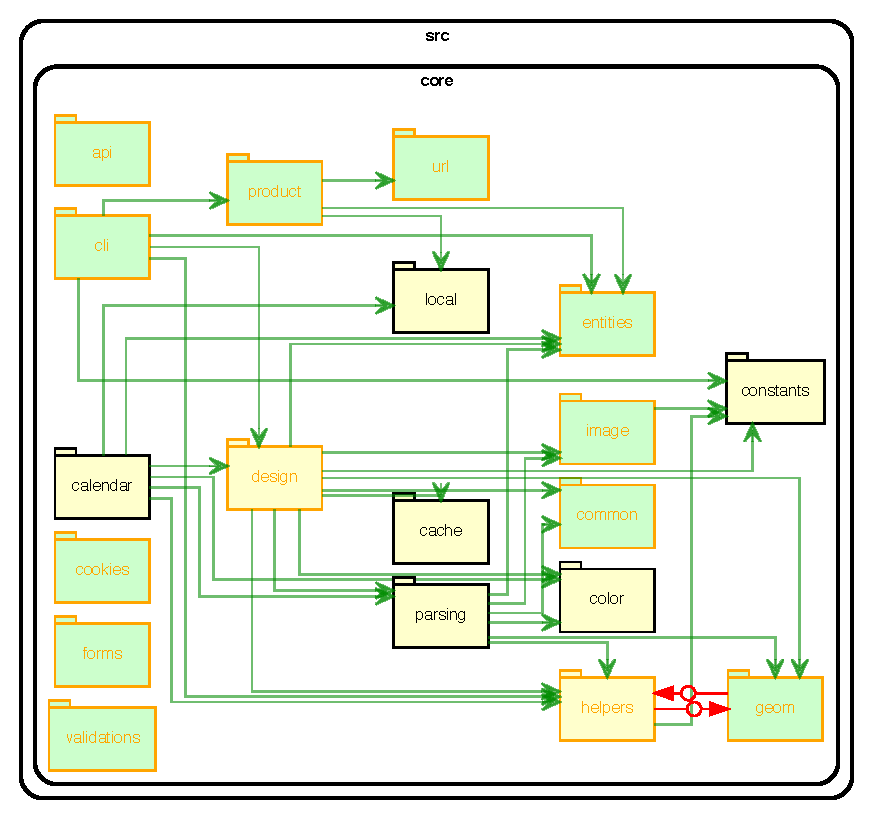
\includegraphics{diagrams/Ist-Architektur/core-graph.pdf}
% 	\caption{Übersicht  }
% 	\label{fig:coreGraph}
% \end{figure}

